\documentclass[12pt]{article}
\usepackage{amsmath}
\usepackage{graphicx}
\graphicspath{ {images/} }
\usepackage{hyperref}
\usepackage{pgfgantt}
\usepackage{rotating}
\usepackage[utf8]{inputenc}
\usepackage[backend=biber, style=authoryear, sorting=nty]{biblatex}
\renewcommand*{\nameyeardelim}{\addcomma\space}
\addbibresource{bibliography.bib}

\title{%
  Building a programming language without the dependency on English \\
  \large CMP6102 Individual Project:
 Project Proposal }

\author{Pandelis Zembashis | S15101590 \\ 
Supervisor: Emmmett Cooper}

\date{November 2018}

\begin{document}
\maketitle

\clearpage


\section{Introduction and background}

Computer languages are heavily westernised as the majority of 
early innovation around computer science, in the late 50's to 60's 
took place in the west (North America and Europe). Most if not all
modern programming languages can trace their routes back to two of
most influential languages of this time period, ALGOL 68 and COBOL 
\parencite{5396281}. Both of these languages were invented in a time
where all interested parties were English speaking and were inventing
processes that would go on to be used by parties that could communicate
in English at some level. Not to mention that the most common input to this
day is still the qwerty keyboard which is comprised of latin characters.

These early languages have grandfathered in English and the Latin 
character set as the basis for all programming languages we see today. 
This is incredibly limiting to the creativity of a given language,
and the accessibility to non native English speakers or different cultures. 
We have limited ourselves to the symbols available to a character set that was not designed with the intention
to be used to program.

\section{Aim}

As a bilingual Computer Science student myself I have experienced the difficulties understanding and adapting to various programming
languages first hand. I also have an avid interest in teaching people how to code. As a founding member of the BCU Hackathon and Computing Society \parencite{noauthor_hacs_nodate}
I have ran many programming workshops for first year computer science students over the last two years. This year I am also a teaching a group of firs time coders
how to code through Code First Girls\parencite{noauthor_code_nodate},
they aim to teach girls with no previous programming experience how to program. I therefore have lots of first hand experience with the
difficulties of both teaching, understanding and learning programming.

Using this experience I hope to put together a language that is more accessible to newcomers and can be used as an educational tool.
While developing the language I can also test attempt to teach it to users and see how they react to it and adapt the language during the development process.


\section{Objectives}

\section{The Product}

I propose a language be designed around its own character set without the dependency on English at its core.
There are alternate writing systems that use logographic character sets where in which a single
character can describe an entire word or phrase, take Chinese and its derivative script Japanese Kanji or Egyptian hieroglyphs for example.
Using this logographic system as inspiration for a language opens up many more creative
avenues for how the language can be designed. 

We can assign any meaning we wish to an arbitrary character
instead of taking a complex set of English words or symbols to create language keywords we can have language symbols dedicated to each task.
Similar to how some programming languages allow for macros, a single instruction that expands automatically into a set of instructions to perform a particular task,
we could assign complex behaviour to single symbols.

Take this example of a fizz buzz program in a traditional language like Javascript \ref{fig:javascript} and pseudocode of a made up logographic language \ref{fig:logographic}.
In this program any numbers divisible by 3 return Fizz, 5 return Buzz and if divisible by both 3 and 5 it returns FizzBuzz.

\begin{figure}[h]
    \caption{Example of fizz buzz program in Javascript}
    \centering
    \begin{verbatim}
                for (var i=1; i <= 20; i++)
                {
                    if (i % 15 == 0)
                        console.log("FizzBuzz");
                    else if (i % 3 == 0)
                        console.log("Fizz");
                    else if (i % 5 == 0)
                        console.log("Buzz");
                    else
                        console.log(i);
                }
    \end{verbatim}
    \label{fig:javascript}
\end{figure}    

\begin{figure}[ht]
    \caption{Pseudocode example of a logographic approach}
    \centering
    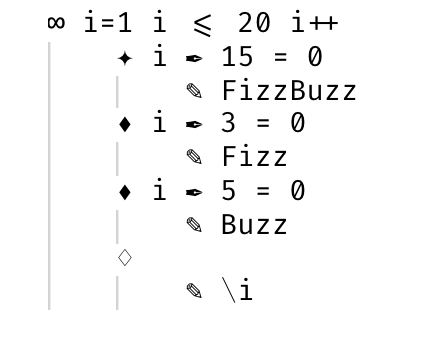
\includegraphics[width=10cm]{logograph}
    \label{fig:logographic}
\end{figure}

\section{Rationale}

I believe that the long lineage of languages being developed on top of a latin character set
has lead to a stagnation in the innovation of languages. Most languages look very similar which is
great for programmers who understand one modern language. It makes picking up a new language pretty easy
when you understand one.

However this dependence on English keywords makes learning your first programming language disproportionately harder
for those without a firm grasp of the English language. This makes learning to program much harder and sometimes
inaccessible to other cultures and languages \parencite{7026875}. 

By creating this language I hope to make a language that is accessible and sensible to users without previous
programming experience. By utilising symbols users only need to learn the meaning of a symbol and not concern themselves
with the difficulty of understanding the characters or cultural nuances \parencite{Eastman:1982:CEN:358728.358756} of another language.


\section{Methodology}


To achieve these goals I hope to create an initial prototype that takes a subset of an existing language like Javascript and transpile from the logographic 
language to a that language to be executed. This will allow me to focus on the designing of the language and quickly prototype a set of symbols that work well together.
During this stage I can use existing language tooling such as Babeljs \parencite{noauthor_babel_nodate} to try out different language semantics. This will enable me to put a working prototype of the language in front of
users in order to validate weather or not the language functions well for its intended purpose.

With a firm set of commands and a basis for the design of the language I can then look towards creating tooling around the language to make it easy to develop in. Finally depending on
the complexity of the first two stages I hope to be able to then create a compiler or virtual machine for the language to run in. I can use an existing compiled language such as GO or a virtual machine like the JVM
to achieve this last stage of developing the language.


\section{Schedule}

\newganttchartelement*{mymilestone}{
mymilestone/.style={
shape=isosceles triangle,
inner sep=0pt,
draw=cyan,
top color=white,
bottom color=cyan!50
},
mymilestone incomplete/.style={
/pgfgantt/mymilestone,
draw=yellow,
bottom color=yellow!50
},
mymilestone label font=\slshape,
mymilestone left shift=0pt,
mymilestone right shift=0pt
}

\newgantttimeslotformat{stardate}{%
\def\decomposestardate##1.##2\relax{%
\def\stardateyear{##1}\def\stardateday{##2}%
}%
\decomposestardate#1\relax%
\pgfcalendardatetojulian{\stardateyear-01-01}{#2}%
\advance#2 by-1\relax%
\advance#2 by\stardateday\relax%
}

\centerline{
\begin{sideways}
\begin{ganttchart}[vgrid, hgrid]{1}{30}
\gantttitle{November}{4} 
\gantttitle{December}{5}
\gantttitle{January}{4}
\gantttitle{Februrary}{4}
\gantttitle{March}{4}
\gantttitle{April}{5}
\gantttitle{May}{4}\\
\gantttitle{Semester 1}{6}
\gantttitle{Holiday}{3}
\gantttitle{1}{1}
\gantttitle{Exams}{3}
\gantttitle{Semester 2}{10}
\gantttitle{Easter}{2}
\gantttitle{Semester 2}{5}\\
\gantttitlelist{7,...,12}{1}
\gantttitlelist{1,...,3}{1}
\gantttitlelist{13}{1}
\gantttitlelist{1,...,3}{1}
\gantttitlelist{1,...,10}{1}
\gantttitlelist{1,2}{1}
\gantttitlelist{11,...,15}{1}\\
%First Group
\ganttgroup{Research}{1}{4} \\
\ganttbar{Literature Review}{1}{4} \\
\ganttbar{Transpilers}{1}{1}
\ganttbar{}{5}{8}\\
\ganttbar{Macros}{2}{2} \\
\ganttbar{Interpreters}{2}{2} \\
\ganttbar{Abstract Syntax Trees}{1}{4} \\
%\ganttlink{elem0}{elem1}
% \ganttlink{elem1}{elem2}
% \ganttlink{elem2}{elem3}
% \ganttmilestone{Milestone 1}{11}
%Second Group
\ganttgroup{Development}{4}{25} \\
\ganttbar{Defining the symbols}{4}{6} \\
\ganttbar{MVP Phase}{5}{10} \\
\ganttbar{Review}{11}{12}\\
\ganttbar{Main Implementation}{13}{18}\\
\ganttbar{Further Development}{20}{24}\\
\ganttlink{elem8}{elem9}
% \ganttlink{elem5}{elem6}
% \ganttlink{elem6}{elem7}
%\ganttmilestone{Milestone 1}{11}
%Third Group
\ganttgroup{Misc}{100}{100} \\
\ganttbar{Industry Presentation}{18}{21} \\
\ganttbar{Poster \& Demo design}{26}{30} \\
\ganttbar{Report}{3}{25} \\
%\ganttlink{elem8}{elem9}
\ganttlink{elem9}{elem10}
\ganttlink{elem10}{elem11}
\ganttlink{elem11}{elem12}
%\ganttmilestone{Milestone 1}{11}
\end{ganttchart}
\end{sideways}}


\clearpage
\printbibliography

\end{document}
